\chapter{Flame Height, Plume Temperature and Ceiling Jets}

\section{Flame Height}

Flame height is recorded by visual observations, photographs, or video footage.  Videos from the NIST/NRC test series and photographs from the VTT Large Hall Test Series are available.  It is difficult to precisely measure the flame height, but the photos and videos allow one to make estimates accurate to within a pan diameter.

\subsubsection{VTT Large Hall Test Series}

The height of the visible flame in the photographs has been estimated to be between 2.4 and 3 pan diameters (3.8 m to 4.8 m).  From the CFAST calculations, the estimated flame height is 4.3 m.

\subsubsection{NIST/NRC Test Series}

CFAST estimates the peak flame height to be 2.8 m, consistent with the roughly 3 m flame height observed through the doorway during the test.  The test series was not designed to record accurate measurements of flame height.

\subsubsection{NIST/Navy High Bay Hangar Test Series}

For the 9 Iceland tests, CFAST predicts flame height within 25~\% of the experimentally reported values, with the largest relative differences for the smaller heat release rate fires. Uncertainty in the flame height measurements for the experiments was reported to be $\pm$ 0.5 m, approaching 30~\% of the experimental values for the lower heat release rate fires.

\section{Plume Temperature}

As with the ceiling jet, CFAST includes a specific plume temperature model based on the McCaffrey plume \cite{Baum:1989, McCaffrey:1983} to account for presence of higher gas temperatures near a target located at the centerline of the fire plume. the correlation has been subjected to extensive validation efforts by McCaffrey \cite{Baum:1989} and others \cite{Valid:Davis_Plumes} and shown to provide predictions within about 30 \% of a wide range of experimental results \cite{Valid:Davis_Plumes}. In the model, this increased temperature has the effect of increasing the convective heat transfer to the target. Only two of the six test series (VTT and FM/SNL) included measurements of plume centerline temperature.

Figure \ref{fig:Plume_Temp_Scatter} shows a comparison of predicted and measured values for plume temperature. Appendix A provides individual graphs of model and experimental values. All of the comparisons are to the surrounding gas temperature predicted by CFAST. Comparisons to the target surface temperature or target center temperature would be expected to have a smaller relative difference since all the predictions of surrounding gas temperature are higher than experimental measurements. Following is a summary of the accuracy assessment for the ceiling jet predictions in the two test series.

\begin{figure}
\begin{center}
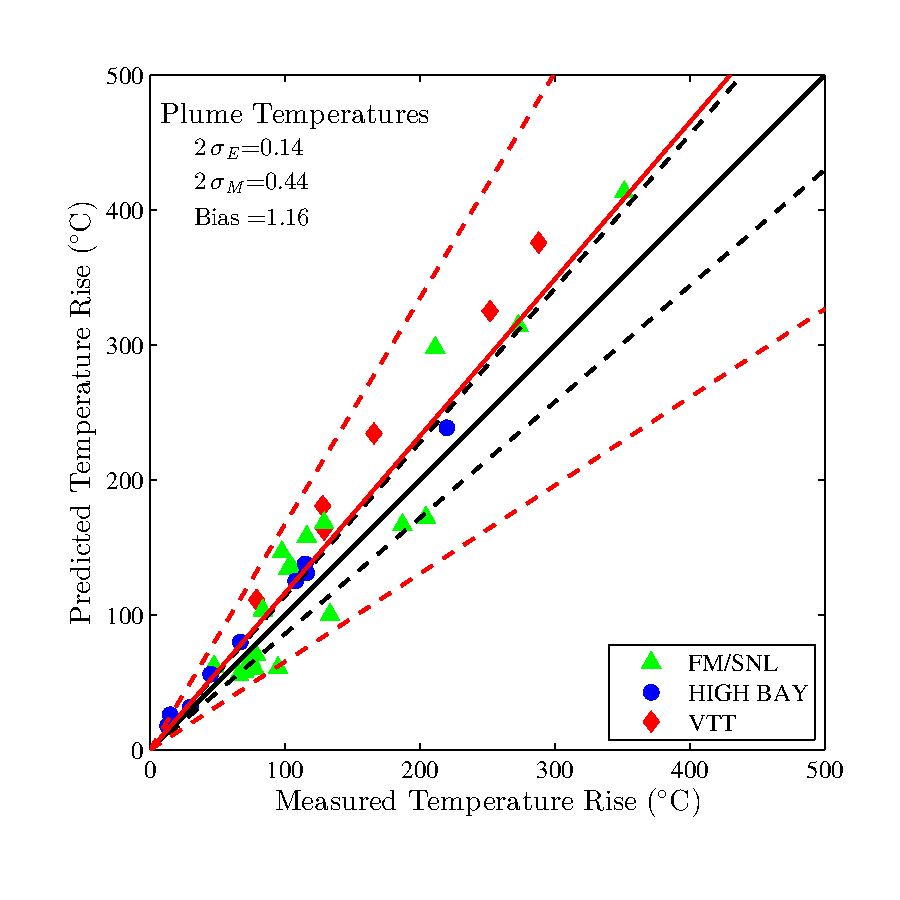
\includegraphics[width=4.0in]{FIGURES/ScatterPlots/Plume_Temperature}  \\
%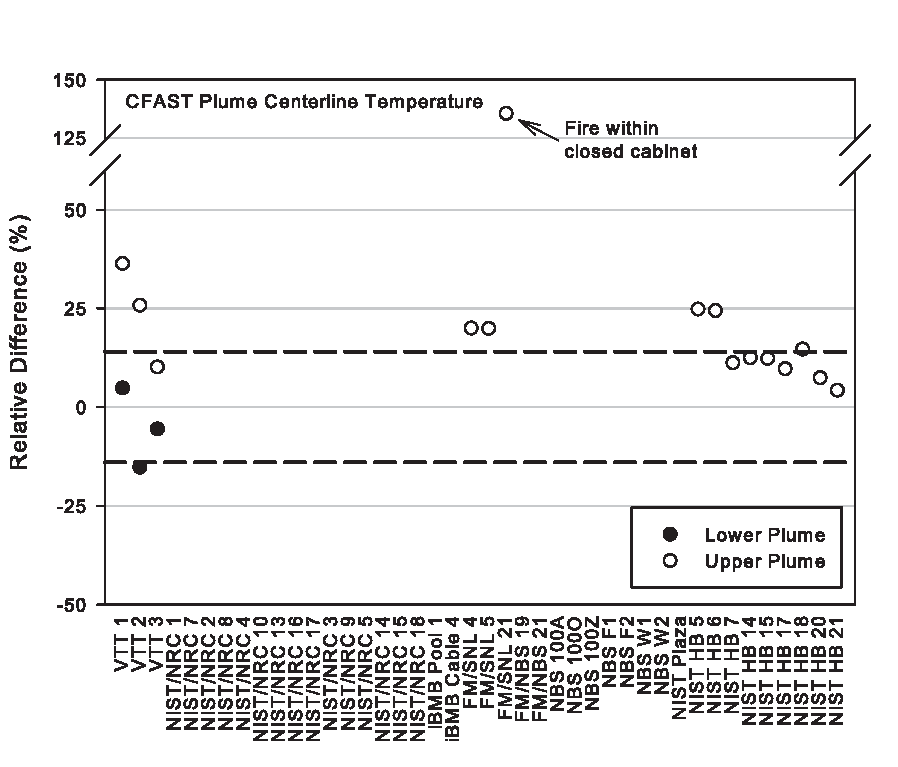
\includegraphics[width=4.0in]{FIGURES/Relative_Diff/Plume_Temps}
\end{center}
\caption{Comparison of Measured and Predicted Plume Centerline Temperature.} \label{fig:Plume_Temp_Scatter}
\end{figure}

\subsubsection{VTT Test Series}

With one exception, CFAST predicts plume temperature within experimental uncertainty for the experiments in this test series. The predictions average within \Plumevtt~\% of the experimental measurements.

\subsubsection{FM/SNL Test Series}

For the tests in this test series, predictions are near experimental uncertainty (averaging within \Plumefmsnl~\% of experimental measurements). This does not include results from test 21 since this test was a fire inside an electrical equipment cabinet that did not form a well-defined plume within the larger compartment.

\subsubsection{NIST / Navy High Bay Hangar Test Series}

Predictions for the high bay tests average within \Plumehighbay~\%.  With a wide range of fire sizes (from 1.4~MW to 33~MW), this test series provides a broad evaluation of the underlying correlations used in the model.  The two tests with the highest relative difference are the lowest heat release rate tests.  With all plume temperature measurements made at a height of more than 22~m, a higher uncertainty for the lowest heat release rate tests is understandable.

\section{Ceiling Jets}

CFAST includes an algorithm to account for the presence of the higher gas temperatures near the ceiling surfaces in compartments involved in a fire.  In the model, this increased temperature has the effect of increasing the convective heat transfer to ceiling surfaces.  The temperature and velocity of the ceiling jet are available from the model by placing a heat detector at the specified location.  The ceiling jet algorithm is based on the model by Cooper \cite{Cooper:1991}, with details described in the CFAST Technical Reference Guide \cite{CFAST_Tech_Guide_6}.  The algorithm predicts gas temperature and velocity under a flat, unconstrained ceiling above a fire source.  Only two of the six test series (NIST/NRC and FM/SNL) involved relatively large flat ceilings.  

Figure \ref{fig:Ceiling_Jet_Scatter} shows a comparison of predicted and measured values for ceiling jet temperature. Appendix A provides individual graphs of model and experimental values. Following is a summary of the accuracy assessment for the ceiling jet predictions in the two test series.

\begin{figure}{t}
\begin{center}
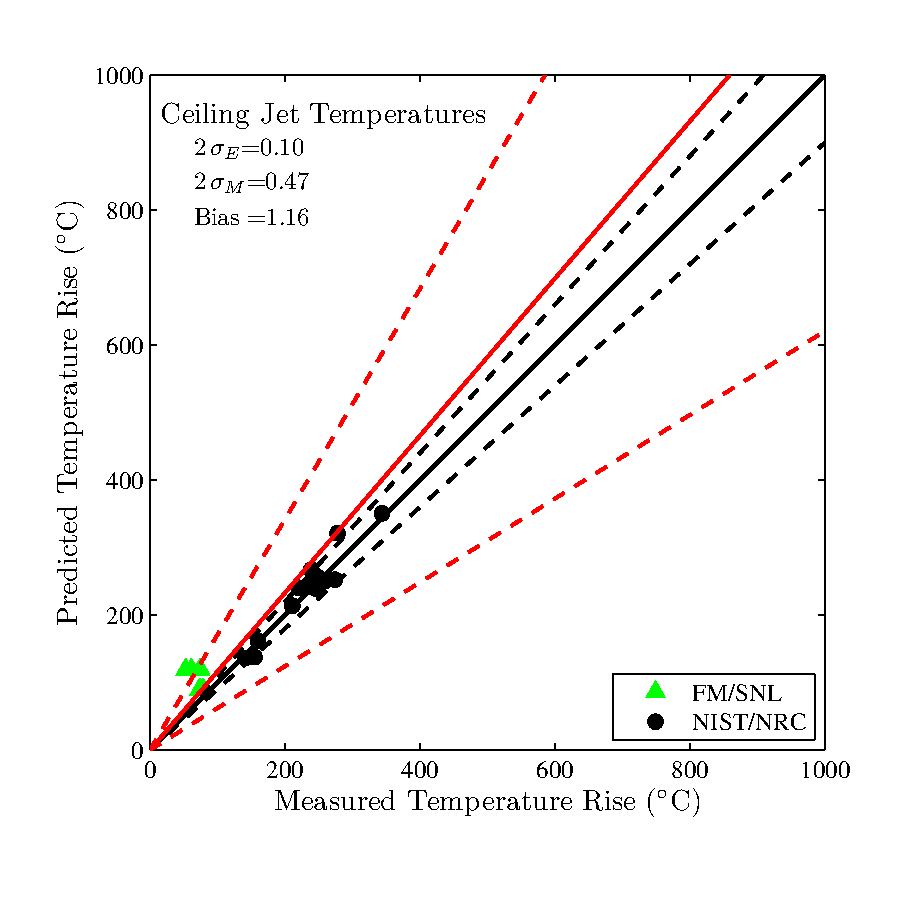
\includegraphics[width=4.0in]{FIGURES/ScatterPlots/Ceiling_Jet_Temperature}  \\
%
\includegraphics[width=4.0in]{FIGURES/Relative_Diff/Ceiling_Jet}
\end{center}
\caption{Comparison of Measured and Predicted Ceiling Jet Temperature.} \label{fig:Ceiling_Jet_Scatter}
\end{figure}

\subsubsection{NIST/NRC Test Series}

The thermocouple nearest the ceiling in Tree 7, located towards the back of the compartment, has been chosen as a surrogate for the ceiling jet temperature. This location was well removed from the fire plume so that plume effects would not be evident, but closer to the wall surfaces so that the assumption of an unconfined ceiling inherent in the typical ceiling jet correlations that wall effects may impact the comparison. Still, CFAST predicts ceiling jet temperature well within experimental uncertainty for all but one of the tests in the series, with an average relative difference of \CeilingJetnistnrc~\%.  For these tests, the fire source was sufficiently large (relative to the compartment size) such that a well-defined ceiling jet was evident in temperature measurements near ceiling level.

\subsubsection{FM/SNL Test Series}

With fire sizes comparable to the smaller fire sizes used in the tests in NIST/NRC test series and compartment volumes significantly larger, measured temperature rise near the ceiling in the FM/SNL tests was below 100~\degc in all three tests. Relative differences averaged within \CeilingJetfmsnl~\% of experimental measurements.  Hot gas layer temperatures for these tests were below 70~\degc.  CFAST consistently predicts higher ceiling jet temperatures in the FM/SNL tests compared to experimental measurements.  With a larger compartment relative to the fire size, the ceiling jet for the FM/SNL tests is not nearly as well-developed as those in the NIST/NRC tests.  The difference between the experimental ceiling jet temperature and HGL temperature for the FM/SNL tests is less than half that observed in the NIST/NRC tests.  While the over-prediction of ceiling jet temperature could be considered conservative for some applications, for scenarios involving sprinkler or heat detector activation, the increased temperature in the ceiling jet would lead to shorter estimates of activation times for the simulated sprinkler or heat detector.

\section{Summary}

Based on the model physics and comparisons of model predictions with experimental measurements, CFAST provides appropriate calculations of flame height for the following reasons:

\begin{itemize}
\item The correlation used in CFAST to predict plume temperature is well-suited for this application and has been subjected to extensive comparisons with experimental results.
\item CFAST provides predictions consistent with visual observation for available data in this validation exercise.
\end{itemize}

Based on the model physics and comparisons of model predictions with experimental measurements, the use of CFAST to predict plume temperature requires caution for the following reasons:

\begin{itemize}
\item The correlation used in CFAST to predict plume temperature is well-suited for this application and has been subjected to extensive validation efforts.
\item CFAST tends to over-predict plume temperatures comparing experimental measurements to gas temperature predictions by the model.  Comparisons to target surface or center temperature (which may be appropriate for unshielded thermocouple measurements in experiments) show closer agreement.
\item 90 \% of the predictions by CFAST are within \Plumeavg~\% of experimental measurements, higher than the estimated experimental uncertainty in this validation exercise, but this is largely driven by a few individual tests.  User's should take this higher uncertainty into account when using predictions from the model.
\end{itemize}

Based on the model physics and comparisons of model predictions with experimental measurements, CFAST provides appropriate calculations of ceiling jet temperature for the following reasons:
\begin{itemize}
\item For tests with a well-defined ceiling jet layer beneath flat ceilings, CFAST predicts ceiling jet temperatures well-within experimental uncertainty.
\item For tests with a less well-defined ceiling jet layer, CFAST over-predicts the ceiling jet temperature.  For the tests studied, over-predictions were noted when the HGL temperature was below 70~$^\circ$C.
\end{itemize}

